\section{问题三：基于连续制氨调节的运行优化}

\subsection{问题分析}

% 本问题将电氢氨装置的运行方式从离散（全开/全停）扩展为连续可调（下限10\%），在24种风光场景下对5种产量水平求解最优功率调度方案\cite{ref4}。连续调节的核心优势在于：设备可以在风光不足时段降低负荷（而非完全停机），减少购电需求的同时维持一定产出，从而在成本和绿电指标之间取得更好的平衡。
本问题将电氢氨装置的运行方式从离散（全开/全停）扩展为连续可调（下限10\%），在24种风光场景下对5种产量水平求解最优功率调度方案。连续调节的核心优势在于：设备可以在风光不足时段柔性降低负荷（而非完全停机），减少高价购电需求的同时维持一定产出\cite{ref4}。此外，为量化连续调节对新能源就地消纳的促进作用，本问题创新性地引入了CCER碳交易机制，将环境生态价值显性化。

\begin{figure}[H]
\centering
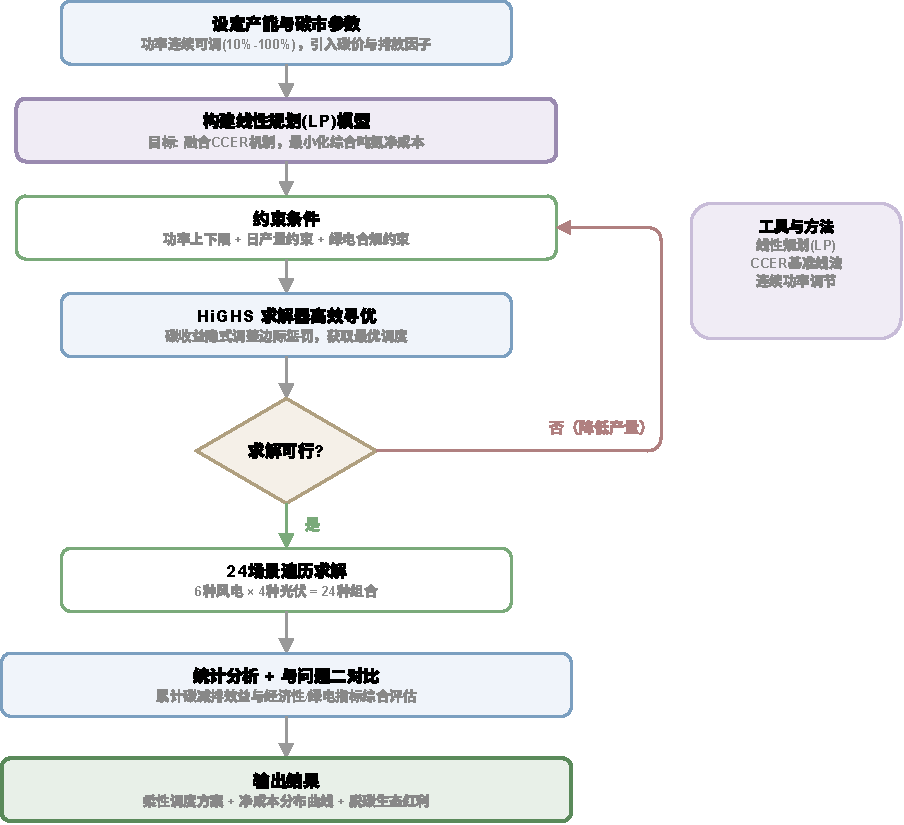
\includegraphics[width=0.85\textwidth,height=0.38\textheight,keepaspectratio]{../figures/fig_flow_q3.pdf}
\caption{问题三求解流程图}\label{fig:flow_q3}
\end{figure}

% 问题三的求解流程如图\ref{fig:flow_q3}所示，将问题建模为标准线性规划（LP），利用HiGHS求解器高效求解。与问题二的贪心算法不同，连续调节引入了时段间的耦合关系（产量约束将所有时段的$\alpha(t)$联系在一起），需要通过LP统一优化。



问题三的求解流程如图\ref{fig:flow_q3}所示。本问题将基础物理拓扑、分时电力市场以及碳减排机制进行全景融合，整体重构为大规模标准线性规划（LP）模型。与问题二的贪心排序算法相比，连续调节不仅引入了时段间的产量耦合约束，更通过碳收益隐式调整了各时段的购售电惩罚权重。最终，利用HiGHS求解器进行统一优化，实现了兼顾经济性与环境生态效益的柔性功率调度。


\subsection{模型建立}

\subsubsection{决策变量与约束}

决策变量为各时段的功率调节系数$\alpha(t) \in [0.1, 1.0]$，$t = 1, 2, ..., 24$。

% 各设备实际功率为额定功率的$\alpha(t)$倍，电氢氨装置总功率$P_{EHA}(t) = 41.5\alpha(t)$ MW。

% 日产量约束为：
% \begin{equation}\label{eq:q3_prod}
% \sum_{t=1}^{24} \alpha(t) \cdot m_{NH3}^{rated} \cdot \Delta t = M_{target} \quad \Rightarrow \quad \sum_{t=1}^{24} \alpha(t) = \frac{M_{target}}{3.0}
% \end{equation}

各设备实际功率为额定功率的$\alpha(t)$倍，电氢氨装置总功率$P_{EHA}(t) = 41.5\alpha(t)$ MW。

日产量约束为：
\begin{equation}\label{eq:q3_prod}
\sum_{t=1}^{24} \alpha(t) \cdot m_{NH3}^{rated} \cdot \Delta t = M_{target} \quad \Rightarrow \quad \sum_{t=1}^{24} \alpha(t) = \frac{M_{target}}{3.0}
\end{equation}

为了量化绿电直连园区的环境生态价值，引入CCER（国家核证自愿减排量）碳交易机制。园区通过消纳本地风光绿电替代传统大电网高碳电力，从而获得碳减排收益\cite{ref6}。$t$时段园区实际消纳的本地绿电功率$P_{RE,used}(t)$可表示为总用电负荷扣除网购电功率：
\begin{equation}
P_{RE,used}(t) = \alpha(t) \cdot P_{EHA}^{rated} + P_{load}(t) - b(t)
\end{equation}

全天流动的日均CCER总减排收益$R_{ccer}$为：
\begin{equation}
R_{ccer} = \sum_{t=1}^{24} P_{RE,used}(t) \cdot \Delta t \cdot e_{grid} \cdot p_{carbon}
\end{equation}
本模型取中国区域电网基准线排放因子$e_{grid} = 0.5703$ tCO$_2$/MWh，基准碳价$p_{carbon} = 70$元/吨。

功率平衡约束为：
\begin{equation}
P_{wind}(t) + P_{pv}(t) + P_{buy}(t) = \alpha(t) \cdot P_{EHA}^{rated} + P_{load}(t) + P_{sell}(t), \quad \forall t
\end{equation}

\subsubsection{线性规划转化}

% 引入辅助变量$b(t) \geq 0$（购电功率）和$s(t) \geq 0$（售电功率），约束$b(t) - s(t) = \alpha(t) \cdot P_{EHA}^{rated} - P_{net}(t)$，其中$P_{net}(t) = P_{wind}(t) + P_{pv}(t) - P_{load}(t)$为已知量。目标函数线性化为：
% \begin{equation}
% \min \quad \frac{1}{M_{target}} \sum_{t=1}^{24} \left[ c_{buy}(t) \cdot b(t) - c_{sell} \cdot s(t) + \bar{c}_{om} \cdot \alpha(t) \cdot P_{EHA}^{rated} \right] \cdot 1000 + C_{RE}
% \end{equation}

引入辅助变量$b(t) \geq 0$（购电功率）和$s(t) \geq 0$（售电功率），约束$b(t) - s(t) = \alpha(t) \cdot P_{EHA}^{rated} - P_{net}(t)$，其中$P_{net}(t) = P_{wind}(t) + P_{pv}(t) - P_{load}(t)$为已知量。

结合综合经济效益最大化原则，将CCER减排收益作为负成本项纳入目标函数。由于$P_{RE,used}(t)$关于决策变量$\alpha(t)$和$b(t)$是严格线性的，因此重构后的综合吨氨净成本优化模型依然保持标准线性规划（LP）形式：
\begin{equation}
\min \quad C_{ton}^{net} = \frac{1}{M_{target}} \left( C_{day}^{base} - R_{ccer} \right)
\end{equation}
其中，$C_{day}^{base}$为基础运行净成本：
\begin{equation}
C_{day}^{base} = \sum_{t=1}^{24} \left[ c_{buy}(t) \cdot b(t) - c_{sell} \cdot s(t) + \bar{c}_{om} \cdot \alpha(t) \cdot P_{EHA}^{rated} \right] \cdot 1000 + C_{RE}
\end{equation}
展开后，最终目标函数转换为求如下线性组合的极小值：
\begin{equation}
\min \quad \frac{1}{M_{target}} \sum_{t=1}^{24} \left\{ \left[ c_{buy}(t)\cdot 1000 + e_{grid}\cdot p_{carbon} \right] \cdot b(t) - c_{sell}\cdot 1000 \cdot s(t) + \left[ \bar{c}_{om}\cdot 1000 - e_{grid}\cdot p_{carbon} \right] \cdot P_{EHA}^{rated} \cdot \alpha(t) \right\} + \Xi
\end{equation}
其中 $\Xi = \frac{1}{M_{target}} \left( C_{RE} - \sum_{t=1}^{24} P_{load}(t)\cdot \Delta t \cdot e_{grid}\cdot p_{carbon} \right)$ 为常数项。由上式可见，碳交易机制的引入实际上隐式调整了优化器对“购电”与“负荷调节”的边际惩罚权重，驱使系统自发减少高碳网购电，提升本地绿电消纳比。


决策变量向量$\mathbf{x} = [\alpha(1),...,\alpha(24), b(1),...,b(24), s(1),...,s(24)]^T$共72维，等式约束25个（24个功率平衡+1个产量约束），变量界$\alpha \in [0.1, 1.0]$，$b, s \geq 0$。由于$c_{buy}(t) > 0$且$c_{sell} > 0$，在最小化目标下互补松弛条件自动满足（$b(t)$和$s(t)$不会同时为正），无需额外互斥约束。

\subsection{典型场景求解结果}

典型场景下连续调节的最优调度方案如图\ref{fig:q3_dispatch}所示。

\begin{figure}[H]
\centering
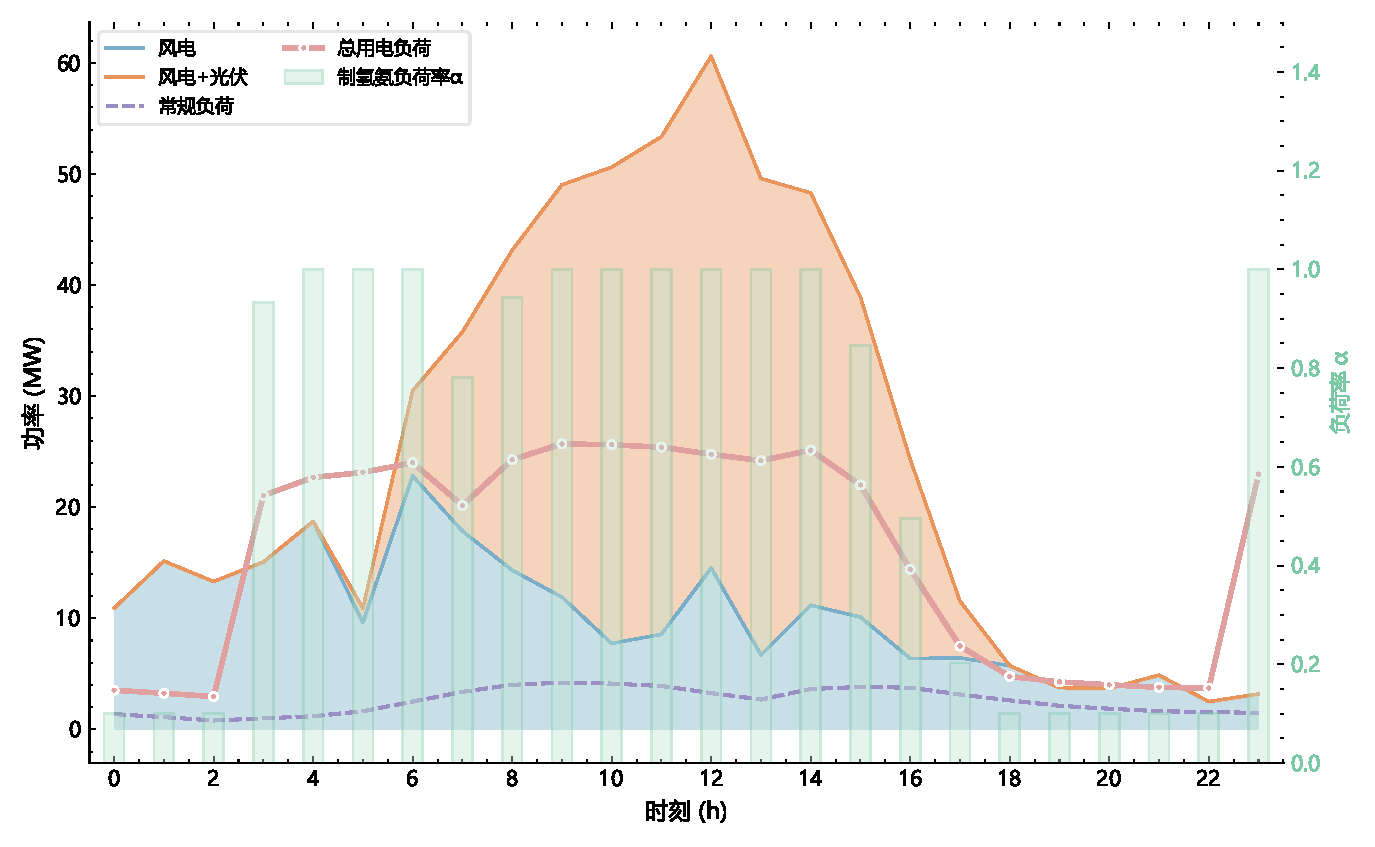
\includegraphics[width=0.85\textwidth,height=0.38\textheight,keepaspectratio]{../figures/fig_q3_dispatch.pdf}
\caption{典型场景连续调度功率分配方案}\label{fig:q3_dispatch}
\end{figure}

连续调度方案展现了"跟踪风光"的特征：在风光充足时段（6:00--16:00）$\alpha(t)$接近或等于1.0（满负荷运行），在风光不足时段（18:00--次日5:00）$\alpha(t)$降至下限0.1附近。这种"削峰填谷"式的负荷调节策略有效减少了购电需求——设备在夜间维持最低运行而非完全停机，避免了停机时段风光余电全部上网导致$R_3$恶化的问题。

\subsection{24种场景全年分析}

\begin{table}[H]
\centering
\caption{问题三24场景连续调节最优方案汇总（部分场景）}\label{tab:q3_scenarios}
\resizebox{\textwidth}{!}{
\begin{tabular}{ccccccc}
\toprule
场景 & 最优产量(吨/日) & 吨氨成本(元/吨) & $R_1$(\%) & $R_2$(\%) & $R_3$(\%) & 达标情况 \\
\midrule
W1P1 & 36 & 2290 & 32.7 & 90.5 & 33.7 & 部分 \\
W1P2 & 36 & 4096 & 81.9 & 81.9 & 9.0 & 全满足 \\
W1P3 & 36 & 5162 & 98.5 & 59.9 & 0.8 & 全满足 \\
W1P4 & 36 & 5808 & 100.0 & 48.8 & 0.0 & 全满足 \\
W2P1 & 36 & 2941 & 30.9 & 77.2 & 34.6 & 部分 \\
W2P2 & 36 & 4668 & 51.8 & 54.4 & 24.1 & 部分 \\
W2P3 & 36 & 6033 & 100.0 & 42.0 & 0.0 & 全满足 \\
W2P4 & 36 & 6940 & 100.0 & 30.4 & 0.0 & 全满足 \\
W3P1 & 36 & 2127 & 33.2 & 93.1 & 33.4 & 部分 \\
W3P2 & 36 & 3869 & 56.3 & 73.1 & 21.8 & 部分 \\
\bottomrule
\end{tabular}}
\end{table}

全年统计结果（表\ref{tab:q3_scenarios}展示部分场景）显示：全满足场景14个，部分满足场景10个，全不满足场景0个。计入碳减排生态红利后，全年加权平均吨氨净成本降至4274.18元/吨。

\subsection{与问题二对比分析}

\begin{table}[H]
\centering
\caption{问题二与问题三关键指标对比}\label{tab:q3_compare}
\begin{tabular}{lccc}
\toprule
指标 & 问题二（离散） & 问题三（连续） & 变化 \\
\midrule
全年吨氨成本 (元/吨) & 4493.82 & 4274.18 & $-$4.9\% \\
全满足场景数 & 0 & 14 & +14 \\
部分满足场景数 & 21 & 10 & $-$11 \\
全不满足场景数 & 3 & 0 & $-$3 \\
\bottomrule
\end{tabular}
\end{table}

问题三相对问题二的改善效果如表\ref{tab:q3_compare}所示，连续调节在经济性和绿电合规性两方面均实现了显著提升。全年吨氨综合净成本降低4.9\%（从4493.82元/吨降至4274.18元/吨），全满足场景从0个增至14个，全不满足场景从3个降至0个。

\begin{figure}[H]
\centering
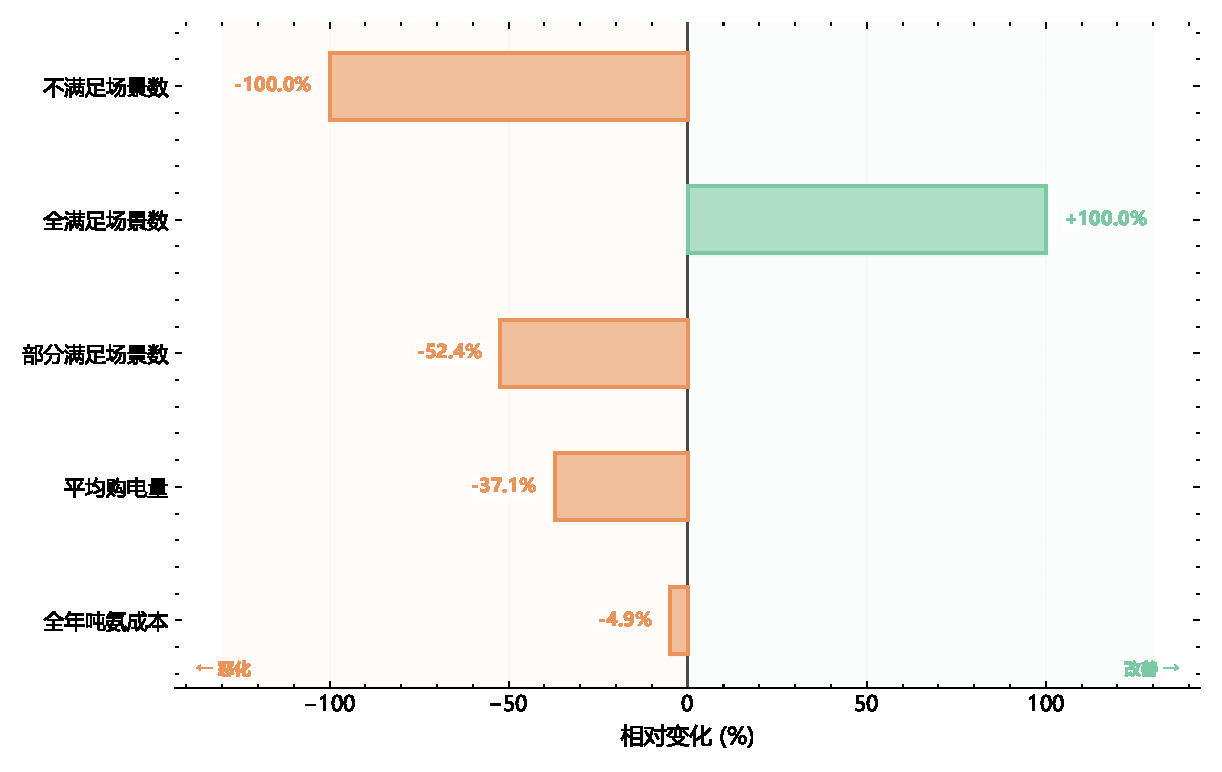
\includegraphics[width=0.85\textwidth,height=0.38\textheight,keepaspectratio]{../figures/fig_q3_compare.pdf}
\caption{问题三相对问题二各指标变化量}\label{fig:q3_compare}
\end{figure}

各指标变化量的对比（图\ref{fig:q3_compare}）进一步揭示了连续调节的优势机制。$R_1$指标改善最为显著，这是因为连续调节在风光不足时段维持最低负荷运行（而非停机），使得设备始终在消纳部分新能源电力，减少了"纯购电"时段的出现。$R_3$指标同样明显改善，原因是设备不完全停机意味着风光余电被部分消纳，上网电量减少。

\begin{figure}[H]
\centering
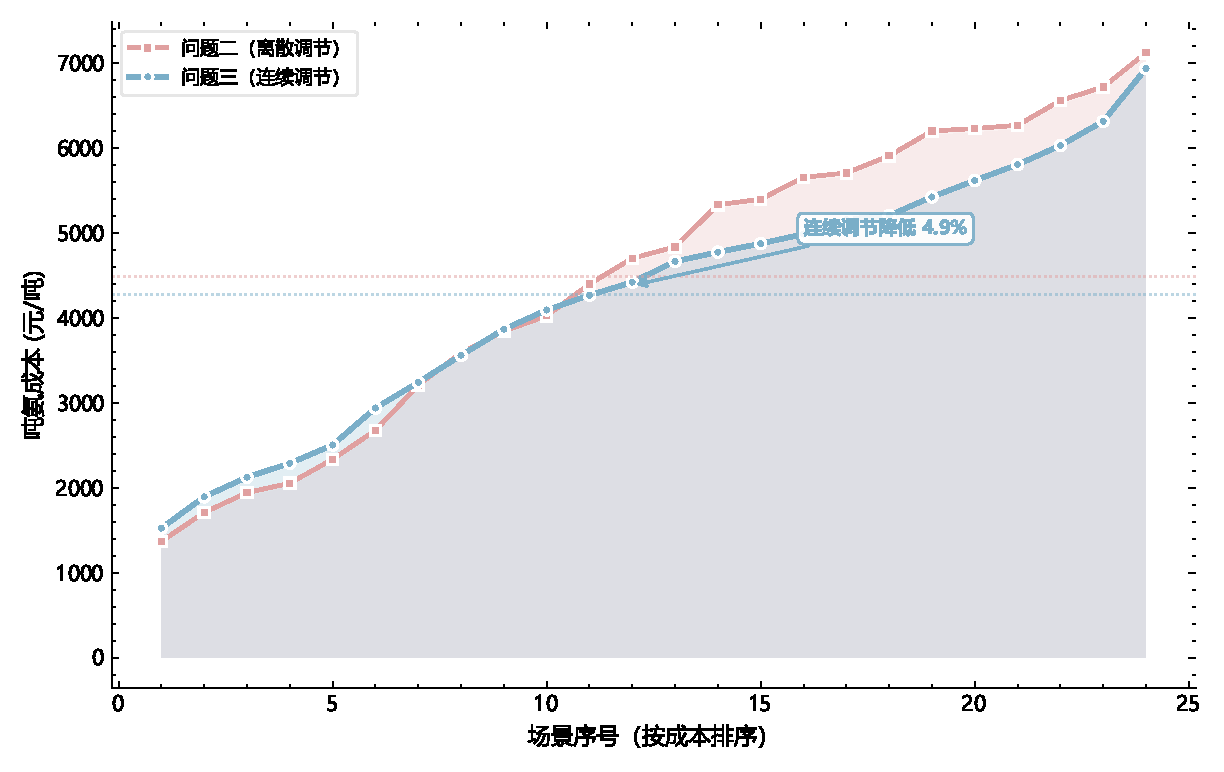
\includegraphics[width=0.85\textwidth,height=0.38\textheight,keepaspectratio]{../figures/fig_q3_annual_cost.pdf}
\caption{全年吨氨成本分布曲线（问题二与问题三对比）}\label{fig:q3_annual_cost}
\end{figure}

全年成本分布曲线对比（图\ref{fig:q3_annual_cost}）显示，连续调节模式下成本分布整体左移（降低），且分布更加集中（标准差减小）。这表明连续调节不仅降低了平均成本，还减小了成本的波动性，使园区运行经济性更加稳定可预期。

连续调节优于离散调节的数学本质在于可行域的松弛关系：问题二的可行解$u(t) \in \{0, 1\}$是问题三可行域$\alpha(t) \in [0.1, 1.0]$的子集（将$u(t)=1$对应$\alpha(t)=1$，$u(t)=0$对应将该时段产量重新分配到其他时段）。因此问题三的最优值必然不劣于问题二。实际改善来源于连续调节允许设备在风光不足时段以低负荷运行，避免了离散模式下"要么全开要么全停"的刚性约束。
